\documentclass{article}

\usepackage{graphicx}
\usepackage{amsmath}
\usepackage{amssymb}
\usepackage{caption}

\renewcommand{\figurename}{Figura}

\begin{document}

\begin{center}
    \Large Banjercito \\[24pt]
    \Large Diplomado en Ciencia de Datos
\end{center}

\vfill

\begin{flushleft}
    \LARGE \textbf{Notas del Curso} \\[12pt]
    \LARGE Módulo III | Semana 3 \\[24pt]
\end{flushleft}

\vfil

\begin{flushleft}
    Instructor: Alan Badillo Salas \\[12pt]
    Agosto 2024 \\[24pt]
\end{flushleft}

\vfill

\section{Introducción}
En la semana 2 estudiamos la varianza de los datos, la cual nace de la idea de ver cuál es el área en la que se aleja un dato del promedio de su eje, al promediar todas las áreas descubrimos un estadístico llamado la varianza, la cual nos permitió obtener un grado de alejamiento cuadrático promedio entre los datos. Al obtener la raíz cuadra de la varianza logramos formar un estadístico adicional llamado la desviación estándar, la cual junto a la media de los datos forman los dos estadísticos principales sobre un eje de datos.
\\[12pt]
Luego extendimos el concepto de la varianza hacia el análisis de dos ejes midiendo su covarianza, es decir, las veces en que un dato se encuentra sobre la media para un eje y si se encuentra sobre la media para el otro eje. Con esto encontramos una relación directa, inversa o nula, para los casos donde los datos de ambos ejes estén por arriba o debajo de su media al mismo tiempo, o de forma inversa o no haya una relación clara entre los cambios.
\\[12pt]
Esta semana estudiaremos las aplicación del análisis de la varianza (\textit{ANOVA}) y las impicaciones que esta tiene en grupos de datos, para determinar si es significativo el grupo al separar un eje de datos. También analizaremos el comportamiento de las cajas estadísticas para asociar los conceptos de las semana anterior.

\clearpage

% \tableofcontents

% \clearpage

\subsection{Contenido de la Semana 3}

Esta semana revisaremos los siguientes temas:

\begin{enumerate}
    \item Análisis por Grupos
    \begin{enumerate}
        \item Segmentación de datos
        \item Media del segmento o clúster
    \end{enumerate}
    \item Visualización por Grupos
    \begin{enumerate}
        \item Datos sobre el Eje
        \item Histogramas
        \item Cajas Estadísticas
    \end{enumerate}
    \item Análisis de la varianza (ANOVA)
    \begin{enumerate}
        \item Intervalo de confianza
        \item Colas 5\% y 95\%
        \item Prueba F de Fisher
        \item Probabilidad de Confusión entre Grupos
    \end{enumerate}
\end{enumerate}

\section{Análisis por Grupos}

Un eje de datos puede ser la edad, la estatura, el peso o el salario de una persona, pero también la altura de un tornillo en una línea de producción, la concentración de gas en un refresco o el monto de crédito aprobado en un préstamo. Un eje por sí mismo no aporta mucha información al análisis global de un estudio, para ello, podemos basarnos en otros ejes para segmentar los datos y encontrar cambios significativos entre los datos.
\\[12pt]
Por ejemplo, vamos a pensar que analizamos el salario de las personas, entonces encontramos que su salario promedio es de \$10,500.00 pesos, esto nos sirve para saber en promedio cuánto gana una persona. Pero ¿Qué pasa si segmentamos los datos en hombres y mujeres? Es decir, ¿Qué pasa si tomamos las muestras que corresponden a aquellas personas que son hombres y por otro lado separamos las muestras de personas que son mujeres?

\subsection{Segmentación de datos}

Cuando separamos los datos de un mismo eje creamos una segmentación, ambos segmentos o grupos tendrán valores relacionados del mismo eje, por ejemplo, si partimos las edades en dos grupos, un grupo será de edades y el otro grupo también, sin embargo, según hagamos la partición los datos podrían tener diferente súmero de elementos, diferente suma, diferente mínimo y máximo, diferente promedio y varianza. Esto significa que la forma de partir o seleccionar grupos es muy importante y determinará la forma en la que analicemos los datos de cada grupo.
\\[12pt]
Si volvemos a la pregunta de qué pasa si segmentamos los datos en hombres y mujeres, la respuesta es que tendremos dos grupos de muestras, un grupo tendrá todas las muestras donde en el eje género sean hombre y otro donde en el género sea mujer. Así, los demás ejes quedarán segmentados y cada partición formará un grupo. Por ejemplo, ahora tendremos un grupo de edades para el segmento de los hombres y otro grupo de edades para el segmento de las mujeres.
\\[12pt]
Entonces los grupos de datos se forman en un eje mediante una segmentación general de las muestras. Cada segmento de muestras formará un grupo para cada eje. Pero, ¿Cómo se comporta la media en cada grupo de cada segmento? ¿Es la misma media la edad promedio en el segmento de mujeres que en el segmento de hombres?

\subsection{Media del segmento o clúster}

Un segmento de muestras es también conocido como un clúster de datos. Recordemos que una muestra es el conjunto de los datos de una persona, o el conjunto de datos de un producto, o el experimento realizado en un laboratorio.
\\[12pt]
Cada muestra contiene información de cada eje, por ejemplo, una muestra de una persona entrevistada en la calle contiene los datos de la edad, la estatura, el peso, el salario, etc. Entonces los bloques de muestras segmentados forman clústeres de análisis, por ejemplo, todas las muestras donde el género es mujer o todas las muestras donde el género es hombre.
\\[12pt]
Diremos que un análisis por clústeres es válido si no hay muestras repetidas entre diferentes clústeres. Por ejemplo, si formamos el clúster de las personas de menos de 18 años y el clúster de las personas mayores a 5 años, entonces los clústeres compartirán muestras y entonces no será un análisis válido, ya que habrá una influencia negativa de las mismas muestras en ambos clústeres, a esto se le llama ruido o redundancia en el análisis.
\\[12pt]
Entonces, para un eje de datos $X$ podemos construir los $k-grupos$ $X_{a}, X_{b}, X_{c}, ..., X_{k}$ donde cada grupo está determinado por una regla de segmentación:
\begin{equation}
    \begin{aligned}
        X_{j} &= \{ x_i \in X | \pi(i, j) \}
    \end{aligned}
\end{equation}
Donde $\pi(i, j)$ es una función que determina si la muestra $i$ pertenecerá al segmento $j$.
\\[12pt]
Así la media de $X_j$ será expresada como $\overline{x^{(j)}}$ y también como $\mu_x^{(j)}$.

\section{Visualización por Grupos}

Ahora vamos a ver de una forma más ilustrativa la implicación de segmentar datos sobre el mismo eje.
\\[12pt]
Imaginemos que tenemos un eje con 150 datos sobre las medidas de la longitud del pétalo de plantas iris (similares a las orquideas). Entonces podríamos visualizar dichos datos sobre un eje dispersando un poco los datos para una mejor visualización:
\begin{figure}[h]
    \centering
    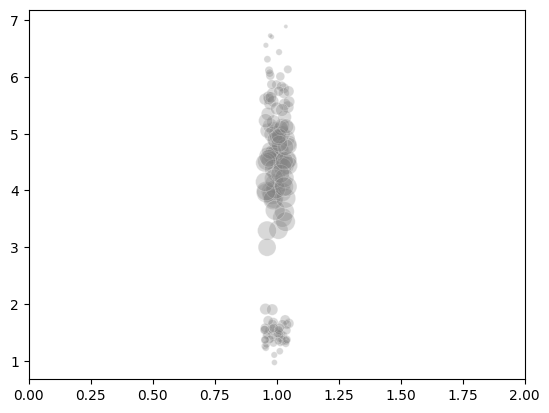
\includegraphics[width=0.6\textwidth]{figures/data1.png}
    \captionsetup{width=0.8\textwidth}
    \caption{Visualización de los datos del eje de la longitud del pétalo para 150 muestras de plantas iris, se alinean al valor de 1 en la coordenada de las absisas y se usan los valores de cada dato para el eje de las ordenadas}
    \label{fig:data1}
\end{figure}
\\
Podemos observar los datos sobre el eje, por ejemplo, algunos están entre el 1 y 2, mientras que los otros están dispersos entre el 3 y el 7. Pero, ¿Qué relación habrá entre los datos dispersos sobre el eje y el segmento o grupo al que pertenecen?

\subsection{Datos sobre el Eje}

Si visualizamos los datos de cada grupo sobre el eje, obtendremos una gráfica similar a la anterior, pero esta vez sabiendo a qué grupo pertenece cada dato, por lo que podemos colorear cada grupo de un color distinto para ubicar más fácilmente los datos sobre el eje.

\clearpage

\hfill\hfill\\
En la Figura \ref{fig:box1} podemos observar los datos sobre eje coloreados por cada grupo en el que se segmentaron los datos.
\begin{figure}[h]
    \centering
    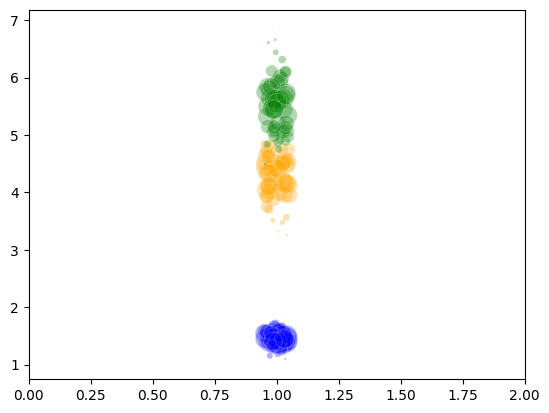
\includegraphics[width=0.6\textwidth]{figures/box1.png}
    \captionsetup{width=0.8\textwidth}
    \caption{Visualización de los datos del eje de la longitud del pétalo para 150 muestras plantas iris, de azul las plantas en el segmento de la setosa, de naranja las versicolor y de verde las virgínicas}
    \label{fig:box1}
\end{figure}
\\
Ahora podemos observar que a diferencia de la Figura \ref{fig:data1} donde los datos son grises y no muestran un comportamiento claro de los datos sobre el eje, al colorearlos por la familia a la que pertenece cada muestra (setosa, versicolor o virginica), podemos entonces visualizar un comportamiento importante en las muestras.
\\[12pt]
Vemos que las muestras que son plantas iris de la familia setosa están al principio del eje, esto significa que las plantas de estas familias tienen un tamaño de pétalo entre 1 y 2 centímetros, mientras que las demás plantas de otras familias tienen mayor tamaño.
\\[12pt]
De forma similar podemos analizar rápidamente la información y descubrir si hay una separación o patrón claro entre los datos, por ejempplo, si tomamos una muestra de una nueva planta iris y su tamaño está entre 1 y 2 centímetros entonces claramente se trata de una setosa, según el comportamiento de los datos.

\clearpage

\hfill\hfill\\
Podemos afinar este análisis mediante una gráfica llamada \textit{Violín} que mostrará la concentración de datos sobre el eje, como sigue:
\begin{figure}[h]
    \centering
    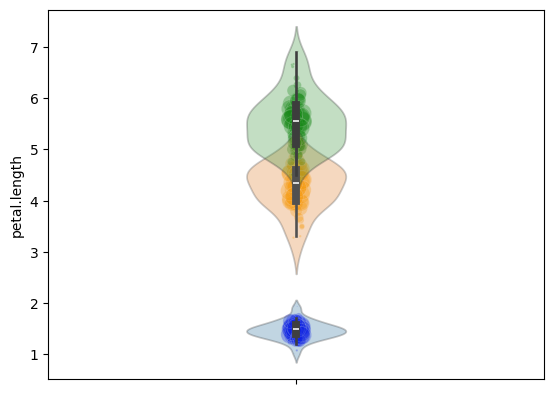
\includegraphics[width=0.6\textwidth]{figures/violin1.png}
    \captionsetup{width=0.8\textwidth}
    \caption{Gráfica de Violín para 150 muestras de la planta iris segmentadas por familia, de azul la familia setosa, de naranja la familia versicolor y de verde la familia virgínica}.
    \label{fig:violin1}
\end{figure}
\\
La gráfica de violín es más útil para visualizar los datos sobre el eje que la gráfica burbujas usada para representar los datos sobre el eje.
\\[12pt]
Con la gráfica de violín no hay necesidad de usar más la otra gráfica, y podemos observar dónde intersectan las dos familias versicolor y virgínica.
\begin{figure}[h]
    \centering
    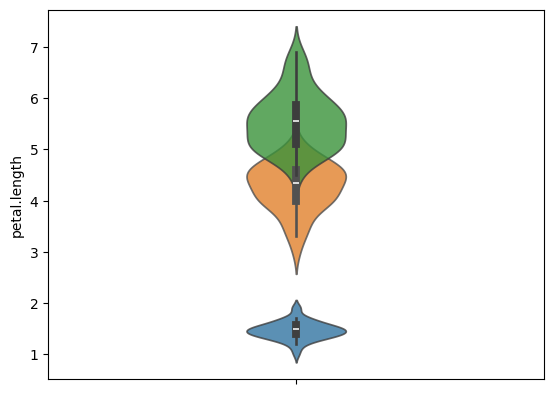
\includegraphics[width=0.6\textwidth]{figures/violin2.png}
    \captionsetup{width=0.8\textwidth}
    \caption{Gráfica de Violín para 150 muestras de la planta iris segmentadas por familia, de azul la familia setosa, de naranja la familia versicolor y de verde la familia virgínica}.
    \label{fig:violin2}
\end{figure}

\clearpage

\hfill\hfill\\
Es interesante observar que si giramos la gráfica de violín 90° obtendremos una gráfica sobre la densidad de los datos de cada grupo:
\begin{figure}[h]
    \centering
    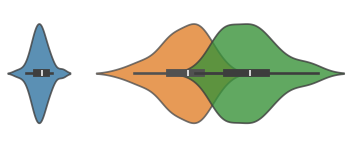
\includegraphics[width=0.6\textwidth]{figures/violin3.png}
    \captionsetup{width=0.8\textwidth}
    \caption{Gráfica de Violín girada 90° para 150 muestras de la planta iris segmentadas por familia, de azul la familia setosa, de naranja la familia versicolor y de verde la familia virgínica}.
    \label{fig:violin3}
\end{figure}
\\
Si además quitamos la simetría obtendremos una gráfica que nos muestra la densidad de cada grupo sobre el eje horizontal.
\begin{figure}[h]
    \centering
    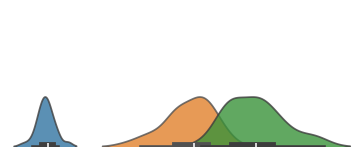
\includegraphics[width=0.6\textwidth]{figures/violin4.png}
    \captionsetup{width=0.8\textwidth}
    \caption{Gráfica de Violín girada 90° y recortada para 150 muestras de la planta iris segmentadas por familia, de azul la familia setosa, de naranja la familia versicolor y de verde la familia virgínica}.
    \label{fig:violin4}
\end{figure}
\\
¿Podemos crear directamente una gráfica similar que nos muestre la misma información?

\subsection{Histogramas}

Los histogramas son conteos sobre el número de datos en intervalos constantes sobre el eje. Es decir, si dividimos el eje desde el valor mínimo, hasta el máximo en $n$-partes iguales, formaremos una especie de cubetas ($bins$ en inglés) o barras que contarán cuántos elementos caen en cada intervalo, de esta manera. 

\clearpage

\hfill\hfill\\
Si graficamos cada barra sabiendo que la altura es el número de elementos en ese intervalo, entonces obtendremos la gráfica de histograma como se muestra:
\begin{figure}[h]
    \centering
    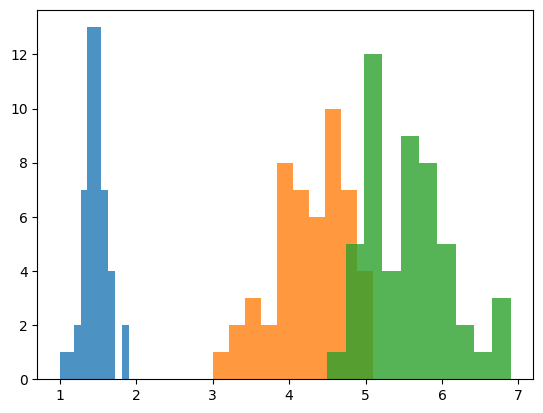
\includegraphics[width=0.6\textwidth]{figures/hist1.png}
    \captionsetup{width=0.8\textwidth}
    \caption{Gráfica de Histograma para 150 muestras de la planta iris segmentadas por familia, de azul la familia setosa, de naranja la familia versicolor y de verde la familia virgínica}.
    \label{fig:hist1}
\end{figure}
\\
En esta gráfica podemos observar los datos de los diferentes segmentos, sobre el eje de la longitud de pétalo y vemos que hay poco más de 12 muestras de la familia Setosa cerca del $1.4$, cerca de 10 muestras de versicolor entre 4 y 5 y poco más de 8 muestras de virgínica cerca del 5.5.
\\[12pt]
Efectivamente la Gráfica de Histograma muestra la densidad o frecuencia de los datos sobre el eje y generalmente donde hay mayor densidad se ubica el promedio o la moda.

\clearpage

\hfill\hfill\\
Si medimos la densidad de los datos en lugar de su frecuencia, entonces para datos más compactos tendremos mayor altura, así por ejemplo, los datos de la Setosa están más densos, por lo que la altura se incrementará:
\begin{figure}[h]
    \centering
    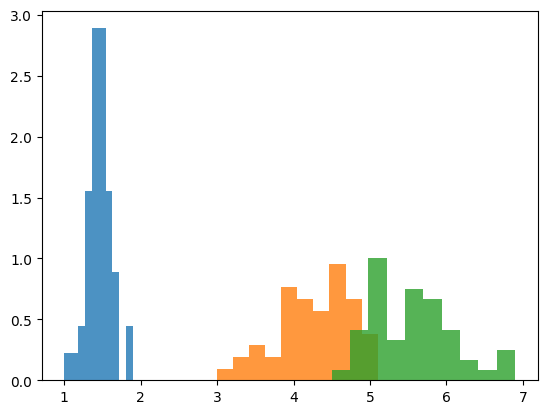
\includegraphics[width=0.5\textwidth]{figures/hist2.png}
    \captionsetup{width=0.8\textwidth}
    \caption{Gráfica de Histograma Denso para 150 muestras de la planta iris segmentadas por familia, de azul la familia setosa, de naranja la familia versicolor y de verde la familia virgínica}.
    \label{fig:hist2}
\end{figure}
\\
El histograma denso ahora muestra picos más pronunciados en datos más pegados, esto es útil para visualizar la distribución densa de los datos:
\begin{figure}[h]
    \centering
    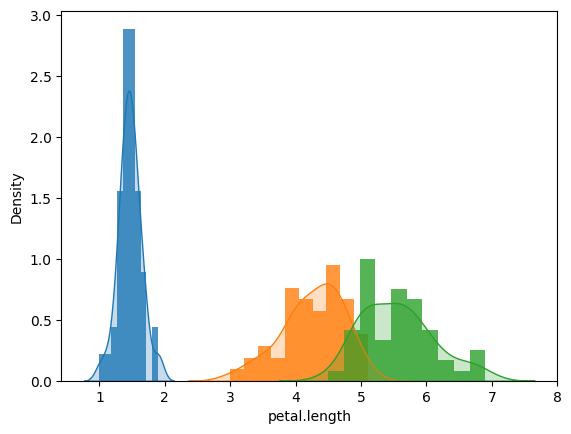
\includegraphics[width=0.5\textwidth]{figures/hist3.png}
    \captionsetup{width=0.8\textwidth}
    \caption{Gráfica de Histograma Denso para 150 muestras de la planta iris segmentadas por familia, de azul la familia setosa, de naranja la familia versicolor y de verde la familia virgínica}.
    \label{fig:hist3}
\end{figure}
\\
Si proyectamos la densidad sobre el histograma, vemos que ya no es necesario ver las barras del histograma que podrían parecer huecas y difíciles de interpretar, en su lugar veremos una mejor visualización con la gráfica densa.

\clearpage

\hfill\hfill\\
La gráfica de densidad es similar al histograma denso y la gráfica de violín y muestra una mejor forma de visualizar la distribución de datos por grupo:
\begin{figure}[h]
    \centering
    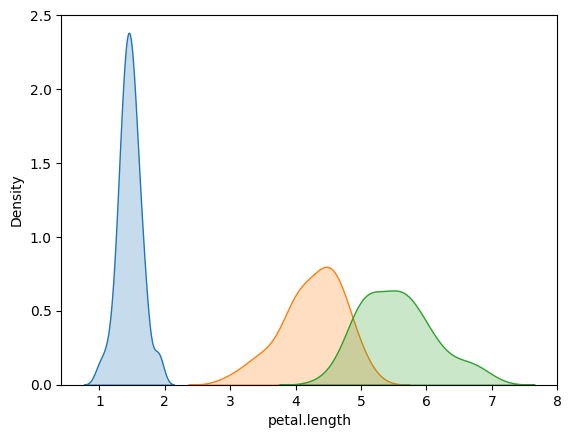
\includegraphics[width=0.6\textwidth]{figures/hist4.png}
    \captionsetup{width=0.8\textwidth}
    \caption{Gráfica de Densidad para 150 muestras de la planta iris segmentadas por familia, de azul la familia setosa, de naranja la familia versicolor y de verde la familia virgínica}.
    \label{fig:hist4}
\end{figure}
\\

\subsection{Cajas Estadísticas}

Si volvemos a analizar los datos sobre el eje, veremos que estos se distribuyen y concentran en distintas partes del eje. Pero, si hay una relación muy fuerte entre los datos del mismo grupo, estos generalmente quedarán contenidos dentro de la caja estadística.
\\[12pt]
La caja estadística está formada por los cuartiles $Q_1 \rightarrow 25\%$, $Q_2 \rightarrow 50\%$ y $Q_3 \rightarrow 75\%$, que representan el promedio para los datos abajo de la media, la mediana y el promedio de los datos arriba de la media respectivamente.
\\[12pt]
Esto significa que podemos formar una caja que encierre al 50\% de la población e indique donde está el valor máximo, el valor mínimo y algunos datos dispersos importantes.
\\[12pt]
La caja estadística es muy útil para saber donde se ubica la mayoría de los datos y es una forma alternativa ala gráfica de violín, histograma y densidad para determinar si dos grupos van a entrar en conflicto o no.

\clearpage

En la siguiente gráfica podemos ver las cajas estadísticas sobrepuestas sobre cada grupo de datos para la longitud de pétalo:
\begin{figure}[h]
    \centering
    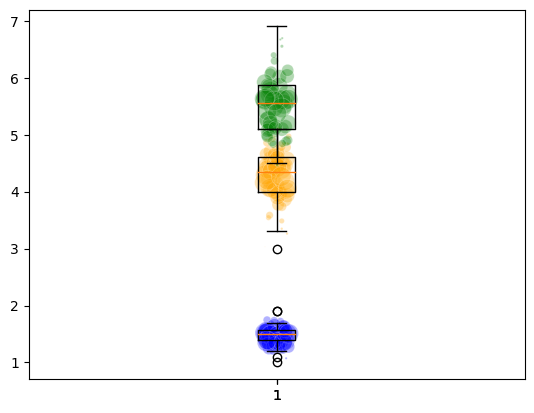
\includegraphics[width=0.5\textwidth]{figures/box2.png}
    \captionsetup{width=0.8\textwidth}
    \caption{Cajas estadísticas sobrepuestas para 150 muestras de la planta iris segmentadas por familia, de azul la familia setosa, de naranja la familia versicolor y de verde la familia virgínica}.
    \label{fig:box2}
\end{figure}
\\
Con estas cajas, nuevamente, ya no es necesario pintar los datos, ya que nos podemos conformar solo con la información de las cajas:
\begin{figure}[h]
    \centering
    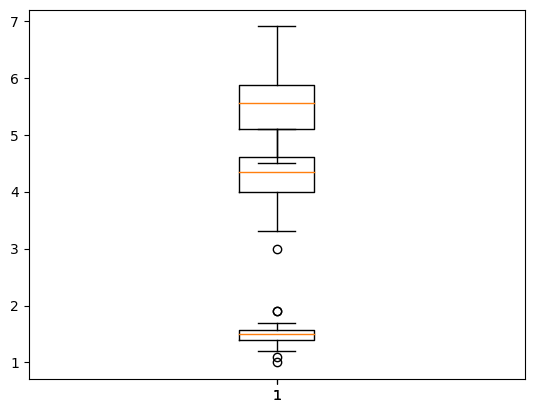
\includegraphics[width=0.5\textwidth]{figures/box3.png}
    \captionsetup{width=0.8\textwidth}
    \caption{Cajas estadísticas para 150 muestras de la planta iris segmentadas por familia, de azul la familia setosa, de naranja la familia versicolor y de verde la familia virgínica}.
    \label{fig:box3}
\end{figure}
\\
Observemos de forma más simple la misma información sobre el eje de datos de los diferentes grupos.

\clearpage

\hfill\hfill\\
Podemos separar las cajas estadísticas para visualizar mejor los datos:
\begin{figure}[h]
    \centering
    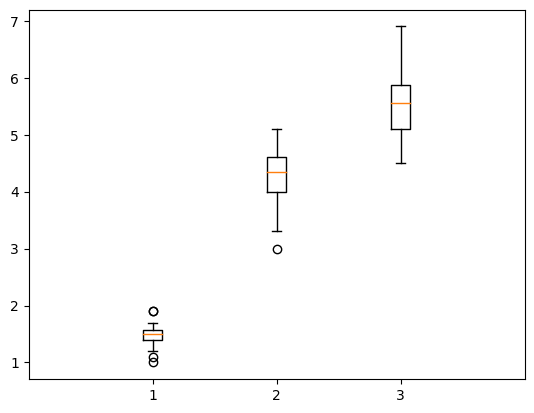
\includegraphics[width=0.5\textwidth]{figures/box4.png}
    \captionsetup{width=0.8\textwidth}
    \caption{Cajas estadísticas separadas para 150 muestras de la planta iris segmentadas por familia, de azul la familia setosa, de naranja la familia versicolor y de verde la familia virgínica}.
    \label{fig:box4}
\end{figure}
\\
También podemos sobreponer nuevamente los datos para ver mejor el comportamiento de cada grupo.
\begin{figure}[h]
    \centering
    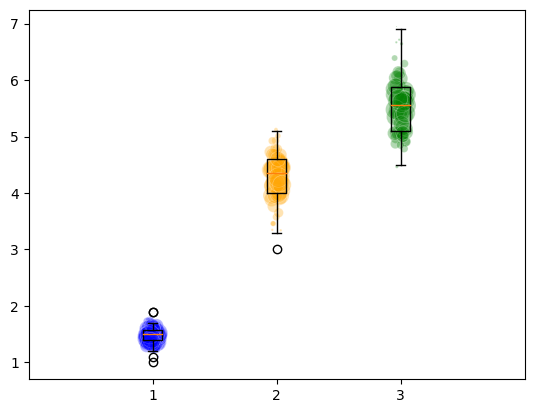
\includegraphics[width=0.5\textwidth]{figures/box5.png}
    \captionsetup{width=0.8\textwidth}
    \caption{Cajas estadísticas separadas y sobrepuestas para 150 muestras de la planta iris segmentadas por familia, de azul la familia setosa, de naranja la familia versicolor y de verde la familia virgínica}.
    \label{fig:box5}
\end{figure}
\\
Pero para no volver tan laborioso el proceso podemos quedarnos con las cajas estadísticas de cada grupo expandidas y coloreadas por grupo.

\clearpage

\hfill\hfill\\
Aquí vemos mejor las cajas estadísticas expandidas:
\begin{figure}[h]
    \centering
    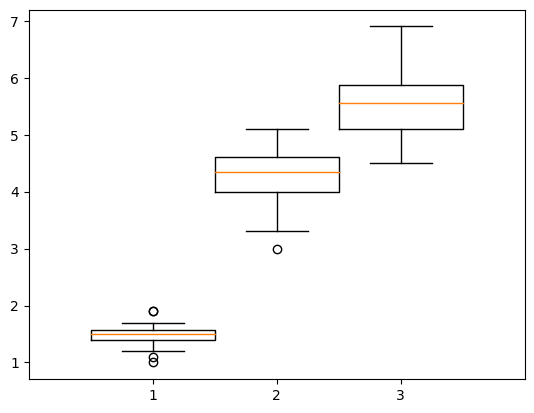
\includegraphics[width=0.5\textwidth]{figures/box6.png}
    \captionsetup{width=0.8\textwidth}
    \caption{Cajas estadísticas separadas y expandidas para 150 muestras de la planta iris segmentadas por familia, de azul la familia setosa, de naranja la familia versicolor y de verde la familia virgínica}.
    \label{fig:box6}
\end{figure}
\\
Y aquí la mejor visualización de las cajas estadísticas separadas, expandidas y coloreadas:
\begin{figure}[h]
    \centering
    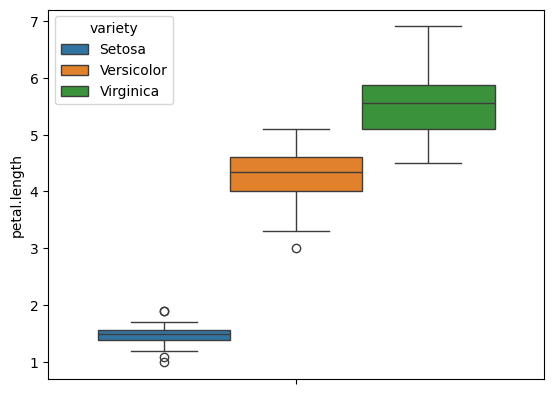
\includegraphics[width=0.5\textwidth]{figures/box7.png}
    \captionsetup{width=0.8\textwidth}
    \caption{Cajas estadísticas separadas, expandidas y coloreadas para 150 muestras de la planta iris segmentadas por familia, de azul la familia setosa, de naranja la familia versicolor y de verde la familia virgínica}.
    \label{fig:box7}
\end{figure}
\\

\section{Análisis de la varianza (ANOVA)}

\subsection{Intervalo de confianza}

\subsection{Colas 5\% y 95\%}

\subsection{Prueba F de Fisher}

\subsection{Probabilidad de Confusión entre Grupos}
    

\end{document}